\FloatBarrier
\section{Overview}

This chapter describes the seven modules added in the second phase of the project, together with the doctor-to-administrator request workflow for beds, the video waiting room, and cancellation with refunds, which were added after the first deployment. Each section states the purpose of the module, the workflow it supports, the rules it enforces, and the most important parts of its implementation. All modules share the platform described in Chapters~\ref{ch:design} and~\ref{ch:impl}: the same authentication and role guards, Zod validation, typed errors, the \texttt{inTransaction} helper, and the notification service. The frontend pages for beds, blood bank, emergency and teleconsultation live in a \texttt{shared/} folder because the same page serves both doctors and administrators; the page hides the actions the current role is not allowed to perform, while the server enforces the same rule independently.

\FloatBarrier
\section{Blood Bank Management}
\label{sec:mod-blood}

\subsection{Purpose and Workflow}

The blood bank module replaces the paper register of a hospital blood bank. Administrators register donors and record each donation, which creates a \emph{unit} of a given component (whole blood, packed red cells, plasma or platelets) with a computed expiry date. Doctors and administrators can see the live inventory grouped by blood group and component, and raise a \emph{request} for a patient, with an urgency of routine, urgent or emergency. An administrator then fulfils the request, at which point the system selects and issues the units, or rejects it with a note. The requesting doctor can cancel a request while it is still pending. Figure~\ref{fig:bloodlife} shows the life cycle of a request and of a unit.

\begin{figure}[H]
\centering
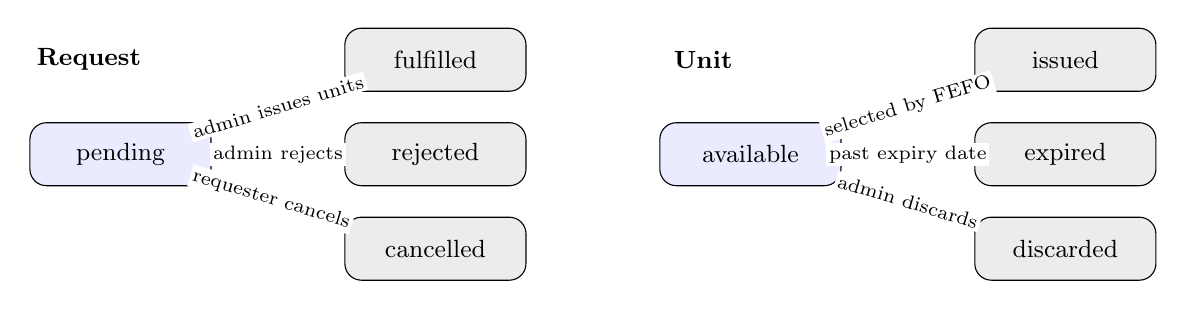
\begin{tikzpicture}[
  st/.style={draw, rounded corners=6pt, minimum width=2.3cm, minimum height=0.8cm, align=center, font=\small, fill=blue!8},
  fin/.style={st, fill=gray!15},
  arr/.style={->, >=stealth, thick},
  lbl/.style={font=\scriptsize, fill=white, inner sep=1pt}
]
\node[font=\bfseries\small] at (-0.4,1.2) {Request};
\node[st] (pend) at (0,0) {pending};
\node[fin] (ful) at (4,1.2) {fulfilled};
\node[fin] (rej) at (4,0) {rejected};
\node[fin] (can) at (4,-1.2) {cancelled};
\draw[arr] (pend) -- node[lbl, sloped]{admin issues units} (ful);
\draw[arr] (pend) -- node[lbl]{admin rejects} (rej);
\draw[arr] (pend) -- node[lbl, sloped, pos=0.45]{requester cancels} (can);

\node[font=\bfseries\small] at (7.4,1.2) {Unit};
\node[st] (av) at (8,0) {available};
\node[fin] (is) at (12,1.2) {issued};
\node[fin] (ex) at (12,0) {expired};
\node[fin] (di) at (12,-1.2) {discarded};
\draw[arr] (av) -- node[lbl, sloped]{selected by FEFO} (is);
\draw[arr] (av) -- node[lbl]{past expiry date} (ex);
\draw[arr] (av) -- node[lbl, sloped]{admin discards} (di);
\end{tikzpicture}
\caption{Life Cycle of a Blood Request and a Blood Unit}
\label{fig:bloodlife}
\end{figure}

\subsection{Business Rules}

\begin{itemize}
    \item \textbf{Compatibility.} Table~\ref{tab:bloodcompat} lists the donor groups that can be issued to each recipient group. Red-cell components use the red-cell ABO table and respect the Rh factor; plasma uses the reversed plasma table and ignores Rh; platelets use the plasma ABO table with the Rh rule \cite{aabb2020}.
    \item \textbf{Exact match first.} Among compatible units, units of the recipient's own group are always issued before substitutes, so that scarce universal-donor O$-$ stock is preserved.
    \item \textbf{First-expiry-first-out (FEFO).} Within the same preference, the unit that expires first is issued first, which minimises wastage.
    \item \textbf{All or nothing.} A request is fulfilled only if enough compatible, unexpired units exist for the full quantity; otherwise nothing is issued and the administrator receives a \texttt{409 Conflict}.
    \item \textbf{Shelf life.} Expiry is computed from the collection date: whole blood 35 days, packed red cells 42 days, plasma 365 days, platelets 5 days. Units past their expiry are marked \texttt{expired} automatically before stock is read or issued.
    \item \textbf{Donor safety.} A donor cannot donate again within 56 days of the previous donation, and a donation date cannot lie in the future \cite{who2012donor}.
    \item \textbf{Alerts.} An emergency-urgency request notifies all administrators, and when an issue leaves fewer than five available units of a group and component, all administrators receive a low-stock alert.
\end{itemize}

\begin{table}[H]
\centering
\caption{Compatible Donor Groups by Recipient and Component (Preferred Order)}
\label{tab:bloodcompat}
\renewcommand{\arraystretch}{1.2}
\begin{tabular}{|C{1.6cm}|L{6.0cm}|L{5.6cm}|}
\hline
\rowcolor{blue!12}
\textbf{Recipient} & \textbf{Whole blood / packed red cells} & \textbf{Plasma} \\
\hline
O$-$  & O$-$ & O$-$, O+, A+, A$-$, B+, B$-$, AB+, AB$-$ \\
\hline
O+    & O+, O$-$ & O+, O$-$, A+, A$-$, B+, B$-$, AB+, AB$-$ \\
\hline
A$-$  & A$-$, O$-$ & A$-$, A+, AB+, AB$-$ \\
\hline
A+    & A+, A$-$, O+, O$-$ & A+, A$-$, AB+, AB$-$ \\
\hline
B$-$  & B$-$, O$-$ & B$-$, B+, AB+, AB$-$ \\
\hline
B+    & B+, B$-$, O+, O$-$ & B+, B$-$, AB+, AB$-$ \\
\hline
AB$-$ & AB$-$, A$-$, B$-$, O$-$ & AB$-$, AB+ \\
\hline
AB+   & AB+, AB$-$, A+, A$-$, B+, B$-$, O+, O$-$ & AB+, AB$-$ \\
\hline
\end{tabular}
\end{table}

\subsection{Implementation}

The compatibility rules are a pure function, \texttt{compatibleDonorGroups(recipient, component)}, which is unit-tested exhaustively for all eight groups and four components. Fulfilment runs inside one transaction: the request row is locked first, expired units are swept, and then the required number of units are selected and locked in a single query whose \texttt{ORDER BY} implements both preferences:

\begin{lstlisting}[language=SQLx, caption=Exact-Group-First FEFO Unit Selection (bloodBankService.js)]
SELECT id FROM blood_units
WHERE status = 'available' AND component = ?
  AND blood_group IN (?)           -- compatible groups only
  AND expires_on >= CURDATE()
ORDER BY (blood_group = ?) DESC,   -- exact match first
         expires_on ASC, id ASC    -- then earliest expiry
LIMIT ? FOR UPDATE
\end{lstlisting}

If fewer rows than requested are returned, the service throws a conflict and the transaction rolls back. Otherwise the units are marked \texttt{issued} with a guarded update (\texttt{WHERE status = 'available'}), the request is marked \texttt{fulfilled}, and after the commit the requesting doctor and the patient are notified. A composite index on \texttt{(status, component, blood\_group, expires\_on)} serves this query. An integration test fires two fulfil requests that compete for the same stock at the same time and checks that exactly one succeeds, one receives \texttt{409}, and neither causes a server error.

\FloatBarrier
\section{Bed Management}
\label{sec:mod-beds}

\subsection{Purpose and Workflow}

Administrators create wards (general, ICU, emergency, maternity, paediatric or private) and beds with a daily rate. The bed board shows every bed with its status (available, occupied, maintenance or reserved) and, for occupied beds, the patient's name and admission time. Each ward card shows total, available and occupied counts, and a statistics panel shows hospital-wide occupancy. Administrators can put a free bed into maintenance or reserve it, but cannot change the status of an occupied bed; an occupied bed becomes free only through discharge. A patient with an open admission cannot be deleted by the administrator.

In a hospital, the decision that a patient needs a bed is clinical, but which bed is free is known to the bed manager. The module follows the same division of work, on the principle of least privilege: \emph{doctors request, the administrator assigns}. Only the administrator can allocate a bed, discharge a patient, or see the full bed grid with patient names. A doctor instead raises a \emph{bed request} for a patient, with a preferred ward type, an urgency (routine, urgent or emergency) and a reason, or a \emph{discharge request} for a patient they admitted. Both kinds of request appear in the administrator's Requests tab, newest emergency first, and inside the Allocate dialog of the bed grid, where requests for the selected bed's ward type are listed first. A bed with a pending discharge request is highlighted in the grid with the requesting doctor, urgency and reason, and its button reads \emph{Approve discharge}. The administrator can also admit a walk-in patient directly from the grid and name an attending doctor.

The doctor whose request led to an admission becomes the \emph{attending doctor} of that stay (\texttt{bed\_allocations.attending\_doctor\_id}). Doctors see only the beds of their own admitted patients, and can request the discharge only of those stays. Figure~\ref{fig:bedreq} shows the life cycle of a request; every change notifies the people involved (Table~\ref{tab:notiftypes}).

\begin{figure}[H]
\centering
\resizebox{\textwidth}{!}{%
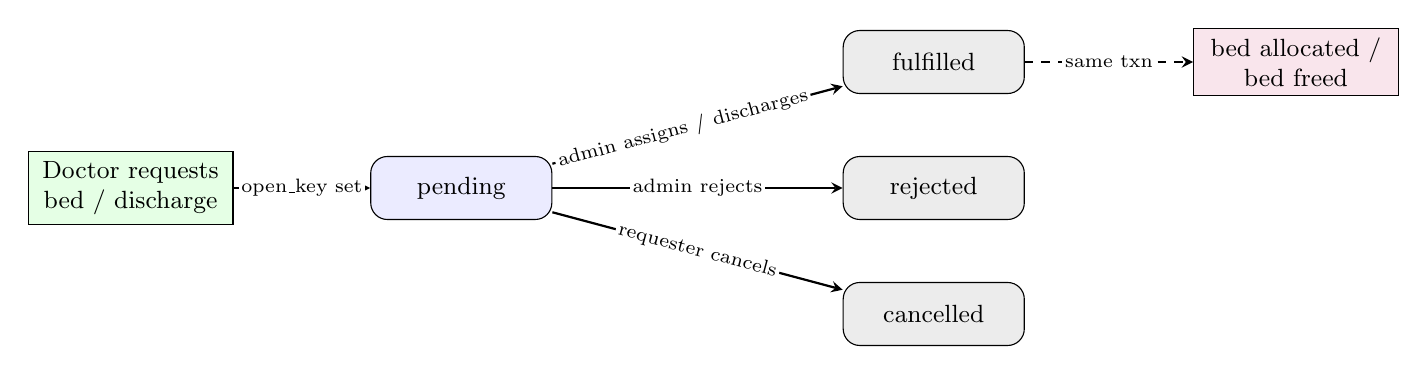
\begin{tikzpicture}[
  st/.style={draw, rounded corners=6pt, minimum width=2.3cm, minimum height=0.8cm, align=center, font=\small, fill=blue!8},
  fin/.style={st, fill=gray!15},
  act/.style={draw, minimum width=2.6cm, minimum height=0.8cm, align=center, font=\small, fill=green!10},
  arr/.style={->, >=stealth, thick},
  lbl/.style={font=\scriptsize, fill=white, inner sep=1pt}
]
\node[act] (doc) at (-4.2,0) {Doctor requests\\bed / discharge};
\node[st] (pend) at (0,0) {pending};
\node[fin] (ful) at (6.0,1.6) {fulfilled};
\node[fin] (rej) at (6.0,0) {rejected};
\node[fin] (can) at (6.0,-1.6) {cancelled};
\node[act, fill=purple!10] (eff) at (10.6,1.6) {bed allocated /\\bed freed};
\draw[arr] (doc) -- node[lbl]{open\_key set} (pend);
\draw[arr] (pend) -- node[lbl, sloped, pos=0.45]{admin assigns / discharges} (ful);
\draw[arr] (pend) -- node[lbl]{admin rejects} (rej);
\draw[arr] (pend) -- node[lbl, sloped]{requester cancels} (can);
\draw[arr, dashed] (ful) -- node[lbl]{same txn} (eff);
\end{tikzpicture}%
}
\caption{Life Cycle of a Bed or Discharge Request}
\label{fig:bedreq}
\end{figure}

\subsection{One Pending Request at a Time}

A patient may have at most one pending admission request, and an admission at most one pending discharge request. As with allocations, the rule is enforced by a unique key rather than by a check alone: \texttt{bed\_requests.open\_key} holds \texttt{admission:<patient id>} or \texttt{discharge:<allocation id>} while the request is pending and is set to \texttt{NULL} when it is fulfilled, rejected or cancelled. A duplicate request therefore fails with \texttt{ER\_DUP\_ENTRY}, which the service turns into a \texttt{409 Conflict}. Assigning a bed for a request locks the request, then the linked emergency case if there is one, and then follows the bed service's lock order (bed, patient, allocation). Assigning from the grid for a patient who has a pending request goes through the same code, so the request is always marked fulfilled and an emergency case is always marked admitted, whichever screen the administrator uses. One subtle point was found by a concurrency test: looking up a missing pending request with \texttt{SELECT \ldots{} FOR UPDATE} on the unique key takes an InnoDB \emph{gap lock} that deadlocks with a doctor's concurrent \texttt{INSERT}. The service therefore reads the key without a lock first and locks the row by its primary key only if it exists.

\subsection{Preventing Double Allocation}

The central correctness requirement is that a bed never has two open allocations and a patient is never admitted to two beds. The application checks both conditions inside a transaction that locks the bed row and the patient's user row (in that fixed order), but application checks alone are not a complete defence: a future code path, a manual SQL statement, or an unforeseen race could still insert a second open row. The guarantee is therefore moved into the schema.

MySQL cannot express ``unique where \texttt{discharged\_at IS NULL}'' directly, and MySQL~8 also forbids a stored generated column over a column that has a cascading foreign key, which rules out the usual computed-column trick. Instead, \texttt{bed\_allocations} has two plain columns, \texttt{open\_bed\_id} and \texttt{open\_patient\_id}, each with a \texttt{UNIQUE} index. They hold the bed and patient ids while the stay is open and are set to \texttt{NULL} on discharge. Because a unique index allows any number of \texttt{NULL} values, closed stays never conflict, while a second open stay for the same bed or patient is rejected by the database itself:

\begin{lstlisting}[language=JavaScript, caption=Allocation Insert Backed by Unique Keys (bedService.js)]
try {
  [ins] = await conn.query(
    `INSERT INTO bed_allocations (bed_id, patient_id, allocated_by,
        attending_doctor_id, reason, open_patient_id, open_bed_id)
     VALUES (?, ?, ?, ?, ?, ?, ?)`,
    [bedId, patientId, allocatedBy ?? null, attending,
     reason ?? request?.reason ?? null, patientId, bedId]);
} catch (err) {
  if (err.code !== 'ER_DUP_ENTRY') throw err;
  throw new ConflictError(/uq_alloc_open_bed/.test(err.message)
    ? 'Bed is not available.' : 'Patient already admitted.');
}
// discharge: SET discharged_at = NOW(), open_patient_id = NULL, open_bed_id = NULL
\end{lstlisting}

The bed's status is then flipped with a guarded update (\texttt{SET status = 'occupied' WHERE id = ? AND status = 'available'}), which can never silently overwrite another state. The migration back-fills the two columns for existing open stays before creating the indexes. Tests check the friendly error messages, a concurrent double admission (one \texttt{201}, one \texttt{409}), and that raw duplicate \texttt{INSERT} statements that bypass the application are rejected by MySQL.

\FloatBarrier
\section{Emergency Management and Triage}
\label{sec:mod-emergency}

\subsection{Purpose and Workflow}

The emergency board is used by doctors and administrators in the emergency department. A new arrival is registered with the patient's name (or linked to an existing registered patient), age, gender, contact, chief complaint, arrival mode (walk-in, ambulance or referral) and vital signs (heart rate, respiratory rate, blood pressure, SpO\textsubscript{2}, temperature). While the form is being filled, the ESI algorithm suggests a triage level, which the clinician can accept or override. The open queue is ordered by triage level and then by arrival time, so that a level 1 patient who arrives last is shown first. Each card can be assigned to a doctor (who is notified), moved into treatment, discharged or transferred. When a registered patient needs admission, the doctor presses \emph{Request bed}, which raises a bed request with emergency urgency and notifies the administrators; the administrator assigns the bed, which admits the case. Only the administrator can admit a case directly into a free bed.

\subsection{ESI Triage Algorithm}

The suggestion follows the ESI version 4 decision points \cite{gilboy2012esi}, shown in Figure~\ref{fig:esi}. It is implemented as a pure function in the backend and duplicated in the frontend for instant feedback; both copies are unit-tested against the same cases.

\begin{figure}[H]
\centering
\begin{tikzpicture}[
  q/.style={diamond, draw, aspect=2.4, align=center, font=\scriptsize, fill=yellow!15, inner sep=1pt},
  l/.style={draw, rounded corners, minimum width=1.6cm, minimum height=0.7cm, font=\small\bfseries, align=center},
  arr/.style={->, >=stealth, thick},
  lbl/.style={font=\scriptsize}
]
\node[q] (a) at (0,0) {Requires immediate\\life-saving intervention?};
\node[q] (b) at (0,-2.0) {High-risk situation, confused,\\or severe pain / distress?};
\node[q] (c) at (0,-4.0) {How many different\\resources needed?};
\node[q] (d) at (0,-6.2) {Danger-zone vitals?\\HR$>$100, RR$>$20, SpO\textsubscript{2}$<$92\%};
\node[l, fill=red!40] (l1) at (5,0) {ESI 1};
\node[l, fill=orange!40] (l2) at (5,-2.0) {ESI 2};
\node[l, fill=yellow!40] (l3) at (-5,-6.2) {ESI 3};
\node[l, fill=green!30] (l4) at (5,-4.0) {ESI 4};
\node[l, fill=blue!20] (l5) at (5,-5.0) {ESI 5};
\draw[arr] (a) -- node[lbl, above]{yes} (l1);
\draw[arr] (a) -- node[lbl, right]{no} (b);
\draw[arr] (b) -- node[lbl, above]{yes} (l2);
\draw[arr] (b) -- node[lbl, right]{no} (c);
\draw[arr] (c) -- node[lbl, above]{one} (l4);
\draw[arr] (c.east) ++(-0.3,-0.25) |- node[lbl, pos=0.75, above]{none} (l5.west);
\draw[arr] (c) -- node[lbl, right]{two or more} (d);
\draw[arr] (d) -- node[lbl, above]{no} (l3);
\draw[arr] (d.east) -- node[lbl, above]{yes} (6.6,-6.2) -- (6.6,-2.0) -- (l2.east);
\end{tikzpicture}
\caption{ESI Version 4 Triage Decision Flow Used for the Suggested Level}
\label{fig:esi}
\end{figure}

\subsection{Status Transitions and Admission}

A case moves through a small state machine (Figure~\ref{fig:erstates}). Only the transitions shown are accepted; any other request, such as reopening a discharged case, returns \texttt{409}. The \texttt{admitted} state cannot be set through the generic update endpoint. It is reached in one of two ways, both inside one transaction that calls the same \texttt{allocateBed} service used by the bed board (so the same lock order and unique keys apply), stores the allocation id on the case and closes it: the administrator's direct admit action, or the administrator assigning a bed for the doctor's emergency bed request. If the case is discharged or transferred while its bed request is still pending, the request is cancelled in the same transaction, and assigning a bed for a request whose case is already closed is refused with \texttt{409}. Registering a case with level 1 or 2 notifies every doctor and administrator.

\begin{figure}[H]
\centering
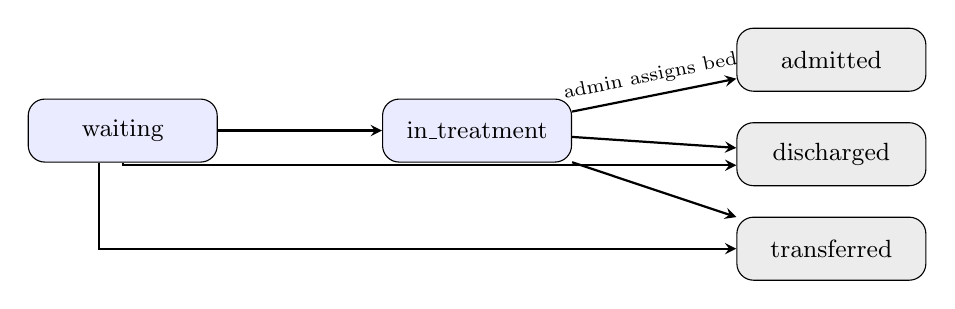
\begin{tikzpicture}[
  st/.style={draw, rounded corners=6pt, minimum width=2.4cm, minimum height=0.8cm, align=center, font=\small, fill=blue!8},
  fin/.style={st, fill=gray!15},
  arr/.style={->, >=stealth, thick}
]
\node[st] (w) at (0,0) {waiting};
\node[st] (t) at (4.5,0) {in\_treatment};
\node[fin] (a) at (9,0.9) {admitted};
\node[fin] (d) at (9,-0.3) {discharged};
\node[fin] (x) at (9,-1.5) {transferred};
\draw[arr] (w) -- (t);
\draw[arr] (t) -- node[font=\scriptsize, above, sloped]{admin assigns bed} (a);
\draw[arr] (t) -- (d);
\draw[arr] (t) -- (x);
\draw[arr] (w.south) |- ([yshift=-4pt]d.west);
\draw[arr] (w.south) ++(-0.3,0) |- (x.west);
\end{tikzpicture}
\caption{Emergency Case Status Transitions}
\label{fig:erstates}
\end{figure}

\FloatBarrier
\section{Teleconsultation}
\label{sec:mod-tele}

\subsection{Purpose and Workflow}

When booking, a patient can choose a video consultation instead of an in-person visit. Video visits require online payment, so they can be booked only when payments are configured. At booking time the server generates a room name of the form \texttt{hms-} followed by 32 random hexadecimal characters (128 bits of randomness), stored in a unique column. At the time of the appointment, the patient and the doctor each open the consultation from their appointment list. The page calls \texttt{GET /api/teleconsult/:appointmentId/join}. The doctor enters the room straight away; the patient enters a \emph{waiting room} instead, as in a real clinic, and is let in only when the doctor clicks \emph{Admit}. After the call, the doctor marks the consultation completed, and the patient is notified.

\subsection{Waiting Room}

Figure~\ref{fig:waitroom} shows the protocol. While the patient waits, the page repeats the join request every five seconds, and each request records the time in \texttt{appointments.video\_waiting\_at}. The doctor's page polls \texttt{GET /status}, which reports the patient as waiting if the last poll was less than 20 seconds ago, so a patient who closed the tab is not shown as waiting. \texttt{POST /admit} sets \texttt{video\_admitted\_at} once; from then on the patient's next join request returns the room details. All three endpoints run the same access checks, and \texttt{/status} and \texttt{/admit} are answered with \texttt{404} for anyone but the appointment's doctor.

\begin{figure}[H]
\centering
\resizebox{\textwidth}{!}{%
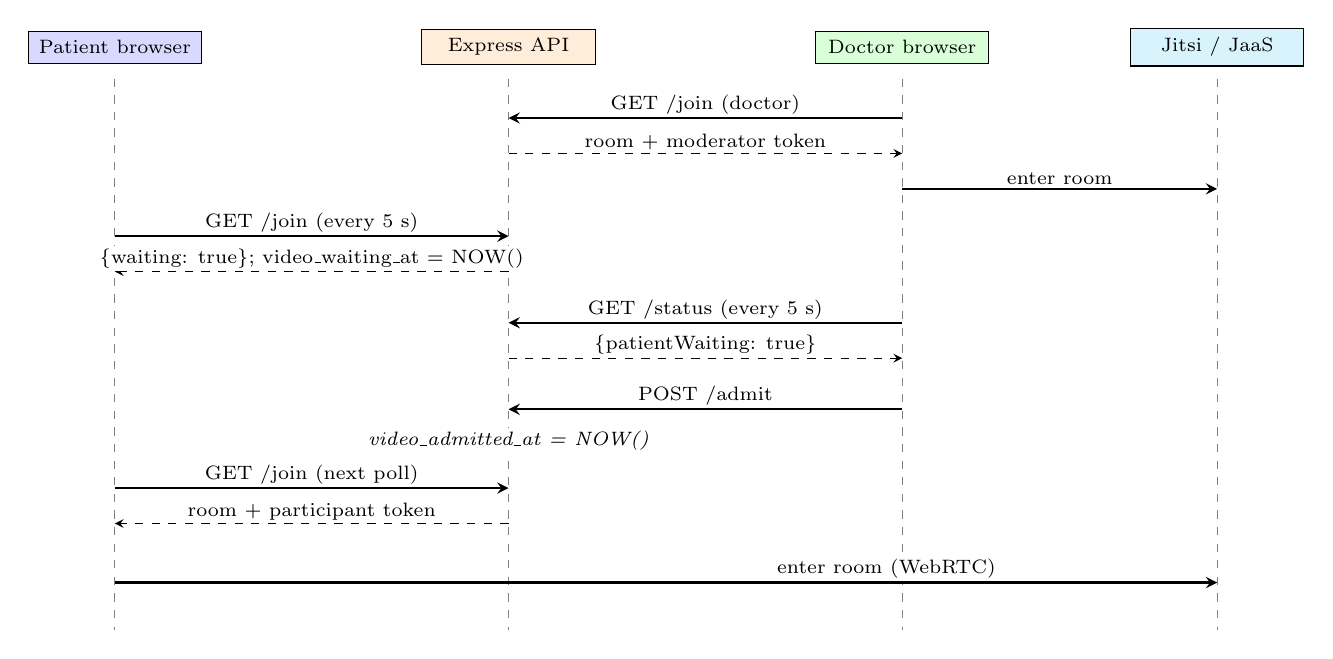
\begin{tikzpicture}[font=\scriptsize, arr/.style={->, >=stealth, thick}, ret/.style={->, >=stealth, dashed}, lb/.style={fill=white, inner sep=1pt}]
\node[draw, fill=blue!15, minimum width=2.2cm] (P) at (0,0) {Patient browser};
\node[draw, fill=orange!15, minimum width=2.2cm] (A) at (5,0) {Express API};
\node[draw, fill=green!15, minimum width=2.2cm] (D) at (10,0) {Doctor browser};
\node[draw, fill=cyan!15, minimum width=2.2cm] (J) at (14,0) {Jitsi / JaaS};
\foreach \x in {0,5,10,14} \draw[dashed, gray] (\x,-0.4) -- (\x,-7.4);
\draw[arr] (10,-0.9) -- node[above, lb]{GET /join (doctor)} (5,-0.9);
\draw[ret] (5,-1.35) -- node[above, lb]{room + moderator token} (10,-1.35);
\draw[arr] (10,-1.8) -- node[above, lb]{enter room} (14,-1.8);
\draw[arr] (0,-2.4) -- node[above, lb]{GET /join (every 5 s)} (5,-2.4);
\draw[ret] (5,-2.85) -- node[above, lb]{\{waiting: true\}; video\_waiting\_at = NOW()} (0,-2.85);
\draw[arr] (10,-3.5) -- node[above, lb]{GET /status (every 5 s)} (5,-3.5);
\draw[ret] (5,-3.95) -- node[above, lb]{\{patientWaiting: true\}} (10,-3.95);
\draw[arr] (10,-4.6) -- node[above, lb]{POST /admit} (5,-4.6);
\node[lb, font=\scriptsize\itshape] at (5,-5.0) {video\_admitted\_at = NOW()};
\draw[arr] (0,-5.6) -- node[above, lb]{GET /join (next poll)} (5,-5.6);
\draw[ret] (5,-6.05) -- node[above, lb]{room + participant token} (0,-6.05);
\draw[arr] (0,-6.8) -- node[above, pos=0.7, lb]{enter room (WebRTC)} (14,-6.8);
\end{tikzpicture}%
}
\caption{Sequence Diagram: Video Waiting Room and Admission by the Doctor}
\label{fig:waitroom}
\end{figure}

\subsection{Access Rules}

Every teleconsultation endpoint applies five checks in order:
\begin{enumerate}
    \item The caller must be the patient who booked the appointment or the doctor assigned to it. Anyone else receives \texttt{404}, so the endpoint does not reveal whether the appointment exists.
    \item The appointment must be a video consultation with a room.
    \item It must still be pending (not completed or cancelled), otherwise \texttt{409}.
    \item A patient must have paid (\texttt{402 Payment Required}); the doctor is not subject to this check.
    \item The current time must be within the join window, from 15 minutes before the start until 60 minutes after it. Outside it the server returns \texttt{403} with the scheduled start time, which the page shows to the user.
\end{enumerate}

The window boundaries are named constants shared with the payment module: a patient can still pay up to 60 minutes after the start, which is exactly as long as the room stays joinable, so a patient is never asked to pay for a consultation they can no longer join.

\subsection{Video Provider and Signed Room Tokens}

During deployment it was found that the public \texttt{meet.jit.si} service no longer allows its rooms to be embedded in third-party websites. The system therefore supports Jitsi as a Service (JaaS, hosted by 8x8 on \texttt{8x8.vc}). When the three variables \texttt{JAAS\_APP\_ID}, \texttt{JAAS\_KID} and \texttt{JAAS\_PRIVATE\_KEY} are set, the join response contains a JSON Web Token signed by the server with the hospital's private key (RS256), valid for two hours and only for that appointment's room. The doctor's token marks them as moderator; recording, live-streaming, transcription and outbound calls are switched off in the token. A person who learns the room name still cannot join without a token, which only the API issues, and only after the checks above. Without the JaaS keys the system falls back to \texttt{JITSI\_DOMAIN}, which is useful for local testing.

\begin{lstlisting}[language=JavaScript, caption=Room-Scoped JaaS Token (utils/videoAccess.js)]
const token = jwt.sign({
  aud: 'jitsi', iss: 'chat', sub: jaas.appId, room, nbf: now - 10,
  context: {
    user: { id: String(user.id), name: user.name, email: user.email,
            moderator: isModerator ? 'true' : 'false' },
    features: { livestreaming: false, recording: false,
                transcription: false, 'outbound-call': false },
  },
}, jaas.privateKey, { algorithm: 'RS256', keyid: jaas.kid, expiresIn: '2h' });
return { domain: '8x8.vc', roomName: `${jaas.appId}/${room}`, jwt: token };
\end{lstlisting}

\FloatBarrier
\section{Notifications and Alerts}
\label{sec:mod-notif}

Notifications are stored in the database and shown through a bell icon in the navigation bar of every signed-in user. The bell shows the unread count, opens a list of the newest notifications, and lets the user open the linked page, mark one notification as read, or mark all as read. The list endpoint supports a limit and an unread-only filter, and is backed by an index on \texttt{(user\_id, is\_read, created\_at)}. A user can only read and update their own notifications; another user's notification id returns \texttt{404}. Table~\ref{tab:notiftypes} lists the events that generate notifications.

\begin{table}[H]
\centering
\caption{Events that Generate Notifications}
\label{tab:notiftypes}
\renewcommand{\arraystretch}{1.2}
\begin{tabular}{|L{2.4cm}|L{5.8cm}|L{5.3cm}|}
\hline
\rowcolor{blue!12}
\textbf{Type} & \textbf{Event} & \textbf{Recipients} \\
\hline
appointment & Appointment booked (form or MediBot) & Patient and doctor \\
\hline
appointment & Appointment cancelled (with refund note if paid) & The other side: doctor if the patient cancelled, patient if the doctor or hospital did, both if the admin did \\
\hline
payment & Payment captured & Patient and doctor \\
\hline
teleconsult & Video consultation completed & Patient \\
\hline
bed & Bed or discharge request raised (doctor or emergency board) & All admins \\
\hline
bed & Request fulfilled (bed assigned or patient discharged) or rejected & Requesting doctor; the patient on admission and discharge \\
\hline
bed & Walk-in admission with a named attending doctor & Patient and attending doctor \\
\hline
emergency & New case with ESI level 1 or 2; case assigned to a doctor & All doctors and admins; assigned doctor \\
\hline
blood & Emergency-urgency request raised; stock of a group/component falls below five units after an issue; request fulfilled & All admins; all admins; requesting doctor and patient \\
\hline
\end{tabular}
\end{table}

As explained in Chapter~\ref{ch:design}, notifications are written after the business transaction commits and their failures are logged, never propagated. Delivery is in-app only; e-mail, SMS and push delivery are listed as future work.

\FloatBarrier
\section{Hospital Navigation}
\label{sec:mod-nav}

\subsection{Purpose and Data Model}

The navigation page is public: a visitor selects a starting point and a destination, optionally ticks ``step-free route'', and receives turn-by-turn directions with the total walking distance and the floor of each step. The hospital is modelled as an undirected weighted graph. Locations (\texttt{nav\_locations}) are nodes with a category, building and floor; connections (\texttt{nav\_edges}) are edges with a distance in metres, a forward and a reverse walking instruction, and an \texttt{accessible} flag that is 0 for staircases. The seeded map covers three floors with 20 locations (entrance, reception, emergency, pharmacy, radiology, lifts, stairs, clinics, wards, blood bank and ICU) and 24 connections. Administrators can add and remove locations and connections.

\subsection{Shortest-Path Algorithm}

For each query the edges are loaded and an adjacency list is built in which every edge is added in both directions with the instruction for that direction. In step-free mode, inaccessible edges are skipped while building the graph, so the search simply cannot use stairs. The route is computed with Dijkstra's algorithm \cite{dijkstra1959}:

\begin{lstlisting}[language=JavaScript, caption=Dijkstra's Algorithm for Indoor Routing (utils/pathfinding.js)]
function shortestPath(graph, fromId, toId) {
  const dist = new Map([[fromId, 0]]), prev = new Map(), done = new Set();
  for (;;) {
    let cur = null;                              // closest unvisited node
    for (const [id, d] of dist)
      if (!done.has(id) && (cur === null || d < dist.get(cur))) cur = id;
    if (cur === null) return null;               // destination unreachable
    if (cur === toId) break;
    done.add(cur);
    for (const e of graph.get(cur) || []) {      // relax neighbours
      const nd = dist.get(cur) + e.distance;
      if (!dist.has(e.to) || nd < dist.get(e.to)) {
        dist.set(e.to, nd);
        prev.set(e.to, { from: cur, instruction: e.instruction, distance: e.distance });
      }
    }
  }
  // walk prev[] back from toId to build the ordered list of steps
}
\end{lstlisting}

The priority queue is a linear scan, giving $O(V^2 + E)$ time. For a hospital map of a few hundred nodes this takes well under a millisecond and avoids extra code; the comment in the source records that a binary heap ($O((V+E)\log V)$) should replace it if the map grows to thousands of nodes. If no route exists (for example a step-free route to a floor with no lift), the API returns \texttt{404} with a clear message rather than an empty list. Unit tests cover shortest-path choice, direction-specific instructions, unreachable targets, the same start and end, and that step-free mode avoids stairs; an end-to-end test drives the public page from Main Entrance to Neurology in both modes.

\FloatBarrier
\section{Online Payments}
\label{sec:mod-payments}

\subsection{Payment Flow}

Patients pay the consultation fee from their appointment history. Figure~\ref{fig:payseq} shows the flow with the Razorpay gateway \cite{razorpaydocs}.

\begin{figure}[H]
\centering
\resizebox{\textwidth}{!}{%
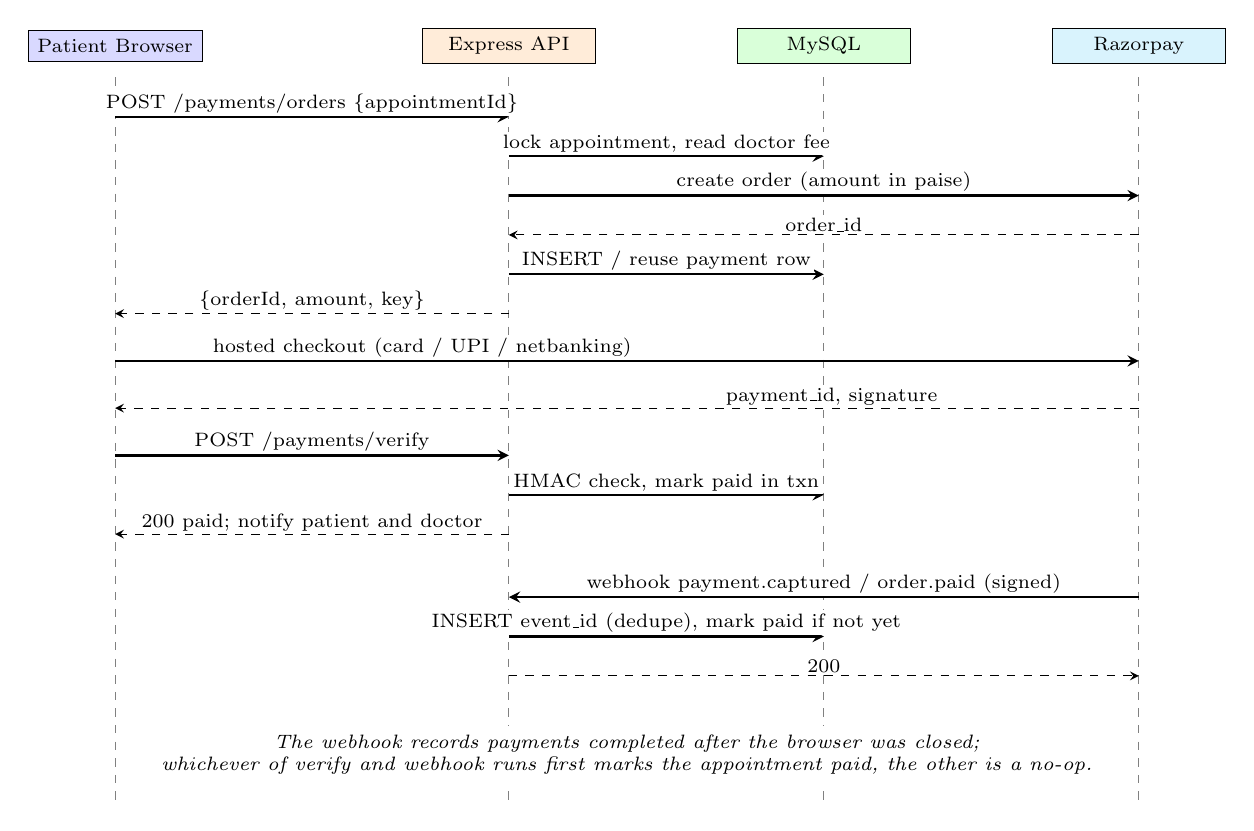
\begin{tikzpicture}[font=\scriptsize, arr/.style={->, >=stealth, thick}, ret/.style={->, >=stealth, dashed}, every label/.style={fill=white}, lb/.style={fill=white, inner sep=1pt}]
\node[draw, fill=blue!15, minimum width=2.2cm, align=center] (B) at (0,0) {Patient Browser};
\node[draw, fill=orange!15, minimum width=2.2cm, align=center] (A) at (5,0) {Express API};
\node[draw, fill=green!15, minimum width=2.2cm, align=center] (D) at (9,0) {MySQL};
\node[draw, fill=cyan!15, minimum width=2.2cm, align=center] (R) at (13,0) {Razorpay};
\foreach \x in {0,5,9,13} \draw[dashed, gray] (\x,-0.4) -- (\x,-9.6);
\draw[arr] (0,-0.9) -- node[above, lb]{POST /payments/orders \{appointmentId\}} (5,-0.9);
\draw[arr] (5,-1.4) -- node[above, lb]{lock appointment, read doctor fee} (9,-1.4);
\draw[arr] (5,-1.9) -- node[above, lb]{create order (amount in paise)} (13,-1.9);
\draw[ret] (13,-2.4) -- node[above, lb]{order\_id} (5,-2.4);
\draw[arr] (5,-2.9) -- node[above, lb]{INSERT / reuse payment row} (9,-2.9);
\draw[ret] (5,-3.4) -- node[above, lb]{\{orderId, amount, key\}} (0,-3.4);
\draw[arr] (0,-4.0) -- node[above, pos=0.3, lb]{hosted checkout (card / UPI / netbanking)} (13,-4.0);
\draw[ret] (13,-4.6) -- node[above, pos=0.3, lb]{payment\_id, signature} (0,-4.6);
\draw[arr] (0,-5.2) -- node[above, lb]{POST /payments/verify} (5,-5.2);
\draw[arr] (5,-5.7) -- node[above, lb]{HMAC check, mark paid in txn} (9,-5.7);
\draw[ret] (5,-6.2) -- node[above, lb]{200 paid; notify patient and doctor} (0,-6.2);
\draw[arr] (13,-7.0) -- node[above, lb]{webhook payment.captured / order.paid (signed)} (5,-7.0);
\draw[arr] (5,-7.5) -- node[above, lb]{INSERT event\_id (dedupe), mark paid if not yet} (9,-7.5);
\draw[ret] (5,-8.0) -- node[above, lb]{200} (13,-8.0);
\node[font=\scriptsize\itshape, align=center, fill=white] at (6.5,-9.0) {The webhook records payments completed after the browser was closed;\\whichever of verify and webhook runs first marks the appointment paid, the other is a no-op.};
\end{tikzpicture}%
}
\caption{Sequence Diagram: Online Payment with Server-Side Verification and Webhook}
\label{fig:payseq}
\end{figure}

\subsection{Security and Correctness Rules}

\begin{itemize}
    \item \textbf{The amount comes from the server.} The client sends only the appointment id; the amount is the doctor's fee converted to paise and read from the database, so it cannot be tampered with.
    \item \textbf{Only payable appointments.} The appointment must belong to the caller, be pending, be unpaid, have a non-zero fee, and not lie more than 60 minutes in the past. The appointment list exposes the same condition as a \texttt{can\_pay} flag computed in SQL, so the \emph{Pay} button is shown exactly when the server would accept the order.
    \item \textbf{Signature verification.} The checkout result is accepted only if \texttt{HMAC-SHA256(key\_secret, order\_id + "|" + payment\_id)} equals the returned signature, compared in constant time to prevent timing attacks. A wrong signature changes nothing.
    \item \textbf{Signed, idempotent webhooks.} The webhook body is verified with the separate webhook secret over the raw request bytes, so the JSON parser is bypassed for this one route. Its event id is inserted into \texttt{payment\_webhook\_events}, whose unique key makes a duplicate delivery a no-op. The webhook is the only state-changing endpoint exempt from CSRF, because it carries no cookies and is authenticated by its signature.
    \item \textbf{Order reuse.} Repeated clicks reuse the existing order while the amount and mode are unchanged, so a patient cannot accumulate several open orders for one appointment.
    \item \textbf{Failing closed.} When Razorpay keys are set, the real gateway is used. Without keys, a mock gateway (with a public test secret) is available only in development and test or with an explicit \texttt{PAYMENT\_MODE=mock}; in production without keys payment returns \texttt{503 Not Configured} rather than silently accepting mock payments.
    \item \textbf{Reconciliation logging.} Rare gateway edge cases, such as a capture on an order that was later replaced, are applied safely and logged with a \texttt{RECONCILE} tag for manual review.
\end{itemize}

\begin{lstlisting}[language=JavaScript, caption=Constant-Time Signature Verification (paymentGateway.js)]
const hmacHex = (secret, data) =>
  crypto.createHmac('sha256', secret).update(data).digest('hex');
function safeEqual(expected, given) {          // never throws
  if (typeof given !== 'string') return false;
  const a = Buffer.from(expected, 'utf8'), b = Buffer.from(given, 'utf8');
  return a.length === b.length && crypto.timingSafeEqual(a, b);
}
function verifyCheckoutSignature(orderId, paymentId, signature) {
  const secret = keySecret();                  // null if payments not configured
  if (!secret || typeof orderId !== 'string' || typeof paymentId !== 'string') return false;
  return safeEqual(hmacHex(secret, `${orderId}|${paymentId}`), signature);
}
\end{lstlisting}

\subsection{Cancellation and Refunds}

Patients, doctors and administrators cancel appointments through one shared service function, so the same rules apply wherever the button is pressed. A patient can cancel only before the start time. Cancelling locks the appointment and then its slot, sets the status to \texttt{cancelled}, clears \texttt{active\_slot\_id} and frees the slot, so that another patient can book it. If the visit was paid, its payment becomes \texttt{refund\_due} and appears in the administrator's ledger; the refund itself is issued from the Razorpay dashboard. If a checkout is still open, its payment row is marked \texttt{failed}, so that a late capture cannot mark a cancelled visit paid; a capture that still arrives for a cancelled visit is stored as \texttt{refund\_due} and logged for reconciliation. After the commit the cached slot list is invalidated and the other side is notified. Payment records also block deletion: the foreign keys from \texttt{payments} to \texttt{appointments} and \texttt{users} are \texttt{ON DELETE RESTRICT}, and the administrator receives a clear \texttt{409} instead of a silent loss of financial history.

\subsection{Payment Views}

Patients see their payment history with status (created, paid, failed or refund due), amount, provider and order/payment ids. Administrators see a ledger of all payments, paginated 50 per page by default (the page size is validated between 1 and 100), together with the total amount collected, the number of paid and pending payments, and the overall count, which drives the page navigation.
